\documentclass[preprint,12pt]{elsarticle}
\usepackage{amsmath,amssymb}
\usepackage{booktabs}
\usepackage{graphicx}
\usepackage[colorlinks=true,linkcolor=blue,citecolor=blue,urlcolor=blue]{hyperref}
\journal{Finance Research Letters}

\begin{document}

\begin{frontmatter}

\title{Anytime-valid monitoring of AI adoption: A real-time signal for technology-linked investment decisions}

\author{Author information removed for double-blind peer review}

\begin{abstract}
Investors and analysts tracking AI-linked technology exposure increasingly consult adoption statistics that update continuously, yet repeatedly testing an accumulating series invalidates the error guarantees of conventional statistics---the same problem that undermines naive interpretation of any live economic dashboard. We apply anytime-valid e-process monitoring, whose type-I error is controlled uniformly over time, to the U.S. Census Bureau's biweekly Business Trends and Outlook Survey of enterprise AI use. The monitor declares a diffusion takeoff on 20 April 2025 (e-value 42.2), quantifies the widely discussed mid-2025 slowdown as sub-threshold evidence later vindicated by re-acceleration, and---using a causal measurement layer that treats survey redesigns as interventions on the observation process---correctly excludes a 25.7-standard-error November 2025 question-wording change that a repeated $z$-test misreads as the largest ``adoption shock'' on record. The framework offers a template for continuously monitoring any adoption-linked exposure without inflating false-signal risk.
\end{abstract}

\begin{keyword}
technology diffusion \sep e-values \sep sequential testing \sep artificial intelligence \sep survey measurement
\end{keyword}

\end{frontmatter}

\section{Introduction}

Real-time adoption statistics now feed investment and allocation decisions as directly as they feed academic research. Since September 2023 the U.S.\ Census Bureau's Business Trends and Outlook Survey (BTOS) has published a biweekly, nationally representative estimate of enterprise AI use \citep{bonney2024}, giving analysts a live read on the diffusion of the technology behind a large share of recent capital expenditure and equity narrative, at a frequency and with a design-based error quantification no comparable general-purpose technology has ever had while it was diffusing. The same is true of any firm's internal adoption telemetry for a new product or platform. The trouble is that dashboards built on such series are inspected continuously, and the classical hypothesis tests underlying most adoption research and most ad hoc dashboard heuristics assume a single test on a closed sample. Applied repeatedly, their error guarantees dissolve: the probability of a false ``regime change'' signal grows without bound in the number of looks \citep{armitage1969}, a fact well known in sequential trial design and rediscovered in industrial experimentation as the peeking problem \citep{johari2022}.

Classical diffusion models---epidemic-style curves \citep{bass1969} and probit-style adoption thresholds \citep{geroski2000}---were built for annual, closed-sample data and estimated once after collection ended; they offer no guidance on how to monitor a live series without accumulating false-alarm risk. Firm-level AI adoption estimates from other instruments range widely, from roughly 5 to 40 percent depending on question wording and sampling unit \citep{crane2025}, which is itself a symptom of the second hazard we address: measurement instruments change. On 17 November 2025 the Census Bureau broadened its AI-use question from production activities to any business function; the published national adoption rate jumped from 10.0 to 17.3 percent overnight---a movement that dwarfs the entire preceding two years of measured diffusion and that a naive monitor would read as an unprecedented shock. Distinguishing a genuine change in adoption from a change in the instrument that measures it is a causal question, not merely a statistical one \citep{pearl2009}, and getting it wrong risks a materially mistaken read on the pace of a technology's diffusion into the economy.

Finance itself has a long tradition of sequential monitoring under continuous inspection---sequential probability ratio tests in trading rule evaluation and CUSUM-style break detection in risk management---but these tools either fix the number and timing of looks in advance or sacrifice a clean error interpretation once monitoring is genuinely open-ended. We address both hazards with a framework built on e-values and anytime-valid inference \citep{shafer2019,vovk2021,ramdas2023}: nonnegative processes that are supermartingales under a null hypothesis of no departure from a baseline path, so that by Ville's inequality the probability of ever crossing a fixed threshold under the null is bounded regardless of how often the series is inspected or when monitoring stops---a guarantee that survives exactly the kind of continuous, unscheduled inspection a live dashboard invites, and that recent work has extended to betting-based and confidence-sequence forms \citep{howard2021,waudbysmith2024}. We combine this with a causal measurement layer that models instrument redesigns as interventions on the observation process, excluding them from the evidence accrual by construction. Applied to the full BTOS AI series, the framework recovers a dated, error-controlled takeoff declaration, correctly treats a subsequent slowdown as inconclusive rather than as a false regime change, and cleanly absorbs the November 2025 redesign that a conventional repeated test misattributes to diffusion. For readers monitoring technology-linked exposures, the exercise is a template: a cheap, one-line construction that lets a live adoption series be watched continuously without manufacturing false signals.

\section{Data and methodology}

We use every published national and firm-size-class BTOS estimate of current AI use, with design-based standard errors, splicing two archived vintages (8 and 15 December 2025) to bridge the November redesign \citep{goldschlag2025}. The result is 56 biweekly national waves: 54 under the original wording (3.7 to 10.0 percent, September 2023 to October 2025) and two under the revised wording (17.3, 17.2 percent).

Let $\hat\pi_t$ be the published adoption-rate estimate with standard error $\hat\sigma_t$, and let $\Delta_t = \hat\pi_t - \hat\pi_{t-1}$. Within a surveillance epoch with baseline slope $\beta$, the standardized increment $z_t = (\Delta_t - \beta)/\sigma_t$ is standard normal under the null that the latent diffusion path continues at rate $\beta$, where $\sigma_t^2 = \hat\sigma_t^2 + \hat\sigma_{t-1}^2$. We run two one-sided Robbins mixture e-processes \citep{robbins1970} on the cumulative sum $S_n=\sum z_t$:
\begin{equation}
E_n^{+} = \frac{2}{\sqrt{a_n}}\,\Phi\!\Big(\frac{S_n}{\sqrt{a_n}}\Big)\exp\!\Big(\frac{S_n^2}{2a_n}\Big), \qquad a_n = n+1,
\label{eq:e}
\end{equation}
with $E_n^-$ defined symmetrically on $-S_n$; both start at 1 and are nonnegative supermartingales under the relevant one-sided null (unit prior scale $\tau=1$). Ville's inequality then gives $\Pr_{H_0}(\exists n: E_n^{+}\ge 1/\alpha')\le\alpha'$, so declaring a shift the first time either monitor reaches $1/(\alpha/2)=40$ controls the false-declaration probability at $\alpha=0.05$ uniformly over time \citep{ramdas2023}---a guarantee that holds whether the series is checked once a year or every wave. After a declaration, the baseline is re-anchored by weighted least squares on the eight preceding waves, opening a new epoch. Pre-announced instrument changes are excluded from the increment sequence by construction, operationalizing the survey redesign as a $\mathrm{do}$-intervention on the observation process rather than on the latent state \citep{pearl2009}; where a break is not pre-announced, a cross-strata check---whether all firm-size classes move together, far outside their own history, in one wave, with a common sign consistent with the mechanical effect of a wording change---separates measurement events from diffusion, in the spirit of invariance-based causal diagnostics \citep{peters2016}. As comparators representing current dashboard practice, we also compute a repeated two-sample $z$-test on four-versus-four-wave windows (uncorrected and Bonferroni-corrected over the running number of looks) and a 3-versus-8-wave moving-average crossing rule, both applied to the naively spliced series exactly as an instrument-unaware analyst would encounter it.

\section{Results}

\begin{figure}[t]
\centering
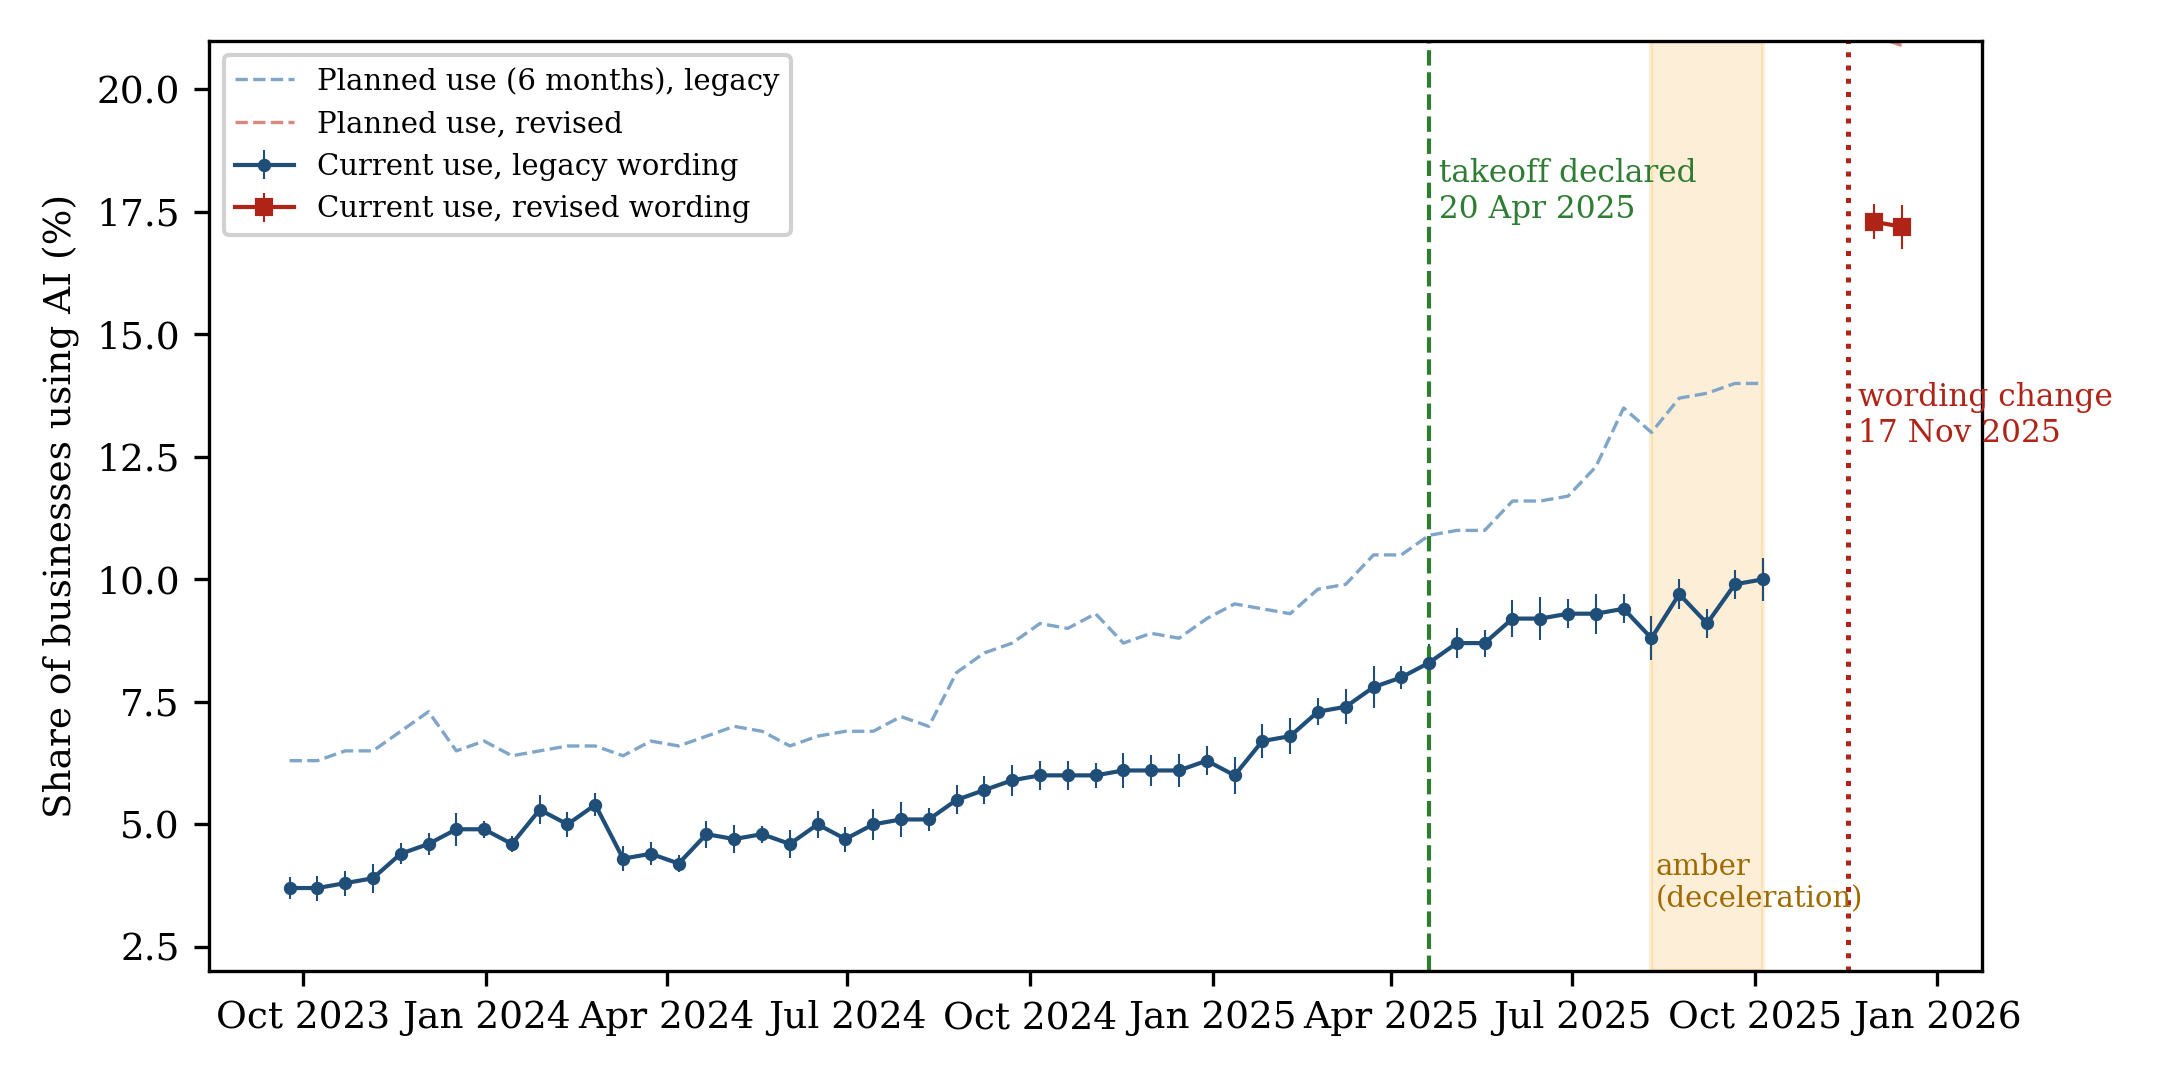
\includegraphics[width=\textwidth]{figure2.png}
\caption{BTOS national AI adoption, September 2023--December 2025. Blue: legacy wording; red: revised wording. Green dashed line: takeoff declaration (20 April 2025); shaded band: deceleration monitor's amber-or-higher span; red dotted line: the excluded question-wording change.}
\label{fig:series}
\end{figure}

Figure~\ref{fig:series} shows the series: a slow 2023--2024 climb, a visible stall through mid-2024, sustained 2025 acceleration, a summer plateau, and the discontinuous jump at the November redesign. Each of these visual features has a corresponding declared or graded statistical event below. Monitoring the null of flat adoption from the second wave, the upward e-process reaches amber ($E\ge2$) by 19 November 2023, peaks at 17.1 on 28 January 2024, retreats to 0.4 by 7 April 2024 during the first-half-2024 growth stall, rebuilds through 2024, and crosses the declaration threshold on \textbf{20 April 2025} with terminal value \textbf{42.2}. The declaration is not premature: it arrives once the acceleration is sustained, not at the first sign of movement, and by Ville's inequality the probability a flat path would ever have produced such a crossing is at most 2.5 percent regardless of how many times the series was checked along the way.

Re-anchoring on the eight waves ending at the declaration fixes a new baseline of 0.299 pp/wave. Against this demanding benchmark, the summer 2025 flattening (8.3 to 8.8 percent) drives the downward monitor to a peak of \textbf{24.3} on 7 September 2025---strong evidence of a slowdown, but short of declaration. Growth resumed to 10.0 percent within weeks, vindicating the restraint: a monitor operated at $\alpha=0.10$ (threshold 20) would have declared a deceleration on 7 September and been contradicted by early October. A repeated four-versus-four-wave $z$-test applied to the same episode whipsaws, crossing on 7 September and reversing on 21 September---two contradictory signals two weeks apart, with no attached error guarantee.

The November redesign is the sharpest test. Between the last legacy wave (10.0 percent) and the first revised wave (17.3 percent) the series jumps 25.7 combined standard errors---against a within-regime history whose largest prior movement is 6.2 standard errors. Because the transition is excluded by construction, the monitor books no diffusion evidence from it. Applied naively (as an unaware dashboard would), a repeated $z$-test posts its largest statistic of the entire sample at this wave ($|z|=32.9$) and alarms both with and without Bonferroni correction---certifying the redesign as the largest ``AI adoption shock'' on record. The contrast is not merely one of counts: the e-process framework yields a single dated event with an attached error rate, while the repeated-testing alternatives yield a signal on the majority of releases, which is functionally equivalent to no signal at all for a reader trying to decide when the underlying process has actually changed. Table~\ref{tab:comp} summarizes. Across all 48 possible looks, the uncorrected $z$-test alarms 37 times over 5 episodes and the Bonferroni-corrected version 31 times over 6---both misfiring at the redesign, where the e-process, by construction, does not.

\begin{table}[t]
\centering
\caption{Detection behavior, September 2023--December 2025 (48 looks).}
\label{tab:comp}
\small
\begin{tabular}{lccc}
\toprule
Method & First alarm & Alarm waves & Alarms at redesign \\
\midrule
Causal e-process ($\alpha=0.05$) & 20 Apr 2025 & 1 & No (excluded) \\
Repeated $z$-test & 14 Jan 2024 & 37 & Yes ($|z|=32.9$) \\
$z$-test, Bonferroni & 14 Jan 2024 & 31 & Yes \\
\bottomrule
\end{tabular}
\end{table}

Firm-size strata corroborate the attribution: all seven employment-size classes---from 1--4 to 250+ employees---jump in the same single wave by 6.1 to 13.8 standard errors, between 2.6 and 7.0 times each class's own within-regime 95th percentile, with a common sign in every case, the signature of an instrument change rather than heterogeneous diffusion. No stratum-level monitor reaches the declaration threshold in-sample; standard errors four to eight times the national series' limit the precision available at that level, and it is the pooled national series where the takeoff is actually earned.

Two sensitivity checks bound the construction. Varying the prior scale $\tau$ between 0.5 and 2 leaves the takeoff declaration on 20 April 2025 for $\tau\in\{0.5,1\}$ and moves it one wave later (4 May 2025) for $\tau=2$; the qualitative pattern of the deceleration episode is unchanged. The null in Eq.~(1) attributes all within-regime dispersion to published sampling error; inflating every standard error by a factor of 1.5---as if additional idiosyncratic noise were present---prevents any in-sample declaration, showing that detection timing is, appropriately, sensitive to that variance assumption even though it is insensitive to the prior.

\section{Discussion and conclusion}

For readers using adoption data to inform technology-linked positioning, three implications follow. First, a dashboard inspected at every release needs anytime-valid statistics, not repeated $t$- or $z$-tests: the difference here is one alarm with a stated error rate versus 31--37 alarms with none. Second, instrument changes in the data an investment thesis relies on---a redefinition, a panel change, a supplement---must be modeled, not assumed away; the causal layer used here is a one-line exclusion rule with a verifiable cross-sectional diagnostic. Third, graded evidence has decision value even without a declaration: the 24.3-to-1 deceleration signal was actionable information that a binary test cannot express, and it correctly stopped short of triggering a reversal that the data would soon contradict. A reader who required a binary call at that moment would have had only the repeated-testing alternative's whipsawing crossings to go on, with no way to tell, from the signal alone, whether either crossing reflected more than noise.

The same construction transfers directly to problems finance researchers already monitor continuously: real-time risk-limit breaches, algorithmic detection of regime change in a return series, or tracking a fintech platform's transaction volume for early signs of adoption stalling or acceleration ahead of a funding or listing decision. In each case the object of interest is a live series inspected at unscheduled intervals, and the choice is the same one this paper makes explicit: either adopt a monitor whose error rate is guaranteed under continuous inspection, or accept that a large but unstated fraction of ``significant'' alerts are artifacts of how often the series was checked.

The exercise has limits. The BTOS is an aggregate biweekly series; firm-level adoption dynamics and their pricing implications require microdata. The framework's sharp null attributes all within-regime dispersion to published sampling error, an assumption that is transparent and adjustable but not costless: an analyst who suspects greater idiosyncratic noise in a series should inflate the variance term accordingly and accept correspondingly later detection, rather than trust a declaration built on an unexamined assumption. The method is demonstrated on one technology in one country through December 2025, with only two post-redesign waves---too few to re-anchor the revised-wording monitor within sample. The cross-strata diagnostic is a screening heuristic with a causal rationale rather than a formally identified estimator, and extending it to settings with less complete stratification (e.g., a single internal product metric with no natural sub-groups to cross-check) would require either a documented change log or an alternative identification strategy. Finally, the choice of $\alpha=0.05$ and a declaration threshold of 40 is a convention imported from the wider anytime-valid literature rather than a value calibrated to any particular decision-maker's cost of a false regime call; a fuller protocol, omitted here for space, would let that threshold be set explicitly to match the asymmetry between acting too early and acting too late. Its promise for finance research is nonetheless direct: any adoption, usage, or transaction series that is watched continuously---AI use, fintech uptake, platform activity---can be monitored with the same time-uniform guarantees, at negligible implementation cost, in place of dashboard heuristics that quietly accumulate false-alarm risk with every look.

\section*{Declaration of competing interest}
The authors declare no known competing financial interests or personal relationships that could have appeared to influence this work.

\section*{Data availability}
All data are public U.S.\ Census Bureau BTOS statistics. The exact analysis dataset and a replication script reproducing every reported number, table, and figure are provided as supplementary material.

\bibliographystyle{elsarticle-harv}
\begin{thebibliography}{00}

\bibitem[{Armitage et~al.(1969)}]{armitage1969}
Armitage, P., McPherson, C.K., Rowe, B.C., 1969. Repeated significance tests on accumulating data. J. R. Stat. Soc. Ser. A 132(2), 235--244. \url{https://doi.org/10.2307/2343787}

\bibitem[{Bass(1969)}]{bass1969}
Bass, F.M., 1969. A new product growth model for consumer durables. Manage.\ Sci.\ 15(5), 215--227. \url{https://doi.org/10.1287/mnsc.15.5.215}

\bibitem[{Bonney et~al.(2024)}]{bonney2024}
Bonney, K., et al., 2024. Tracking firm use of AI in real time. NBER Working Paper 32319. \url{https://doi.org/10.3386/w32319}

\bibitem[{Crane et~al.(2025)}]{crane2025}
Crane, L., Green, M., Soto, P., 2025. Measuring AI uptake in the workplace. FEDS Notes, 5 Feb.\ 2025. \url{https://doi.org/10.17016/2380-7172.3724}

\bibitem[{Geroski(2000)}]{geroski2000}
Geroski, P.A., 2000. Models of technology diffusion. Res.\ Policy 29(4--5), 603--625. \url{https://doi.org/10.1016/S0048-7333(99)00092-X}

\bibitem[{Goldschlag(2025)}]{goldschlag2025}
Goldschlag, N., 2025. How many businesses are using AI? Agglomerations, 19 Dec.\ 2025. \url{https://agglomerations.substack.com/p/how-many-businesses-are-using-ai}

\bibitem[{Howard et~al.(2021)}]{howard2021}
Howard, S.R., Ramdas, A., McAuliffe, J., Sekhon, J., 2021. Time-uniform, nonparametric, nonasymptotic confidence sequences. Ann.\ Stat.\ 49(2), 1055--1080. \url{https://doi.org/10.1214/20-AOS1991}

\bibitem[{Johari et~al.(2022)}]{johari2022}
Johari, R., Koomen, P., Pekelis, L., Walsh, D., 2022. Always valid inference. Oper.\ Res.\ 70(3), 1806--1821. \url{https://doi.org/10.1287/opre.2021.2135}

\bibitem[{Pearl(2009)}]{pearl2009}
Pearl, J., 2009. Causality, 2nd ed. Cambridge Univ.\ Press. \url{https://doi.org/10.1017/CBO9780511803161}

\bibitem[{Peters et~al.(2016)}]{peters2016}
Peters, J., B\"uhlmann, P., Meinshausen, N., 2016. Causal inference by using invariant prediction. J.\ R.\ Stat.\ Soc.\ Ser.\ B 78(5), 947--1012. \url{https://doi.org/10.1111/rssb.12167}

\bibitem[{Ramdas et~al.(2023)}]{ramdas2023}
Ramdas, A., Gr\"unwald, P., Vovk, V., Shafer, G., 2023. Game-theoretic statistics and safe anytime-valid inference. Stat.\ Sci.\ 38(4), 576--601. \url{https://doi.org/10.1214/23-STS894}

\bibitem[{Robbins(1970)}]{robbins1970}
Robbins, H., 1970. Statistical methods related to the law of the iterated logarithm. Ann.\ Math.\ Stat.\ 41(5), 1397--1409. \url{https://doi.org/10.1214/aoms/1177696786}

\bibitem[{Shafer and Vovk(2019)}]{shafer2019}
Shafer, G., Vovk, V., 2019. Game-Theoretic Foundations for Probability and Finance. Wiley. \url{https://doi.org/10.1002/9781118548035}

\bibitem[{Vovk and Wang(2021)}]{vovk2021}
Vovk, V., Wang, R., 2021. E-values: calibration, combination and applications. Ann.\ Stat.\ 49(3), 1736--1754. \url{https://doi.org/10.1214/20-AOS2020}

\bibitem[{Waudby-Smith and Ramdas(2024)}]{waudbysmith2024}
Waudby-Smith, I., Ramdas, A., 2024. Estimating means of bounded random variables by betting. J.\ R.\ Stat.\ Soc.\ Ser.\ B 86(1), 1--27. \url{https://doi.org/10.1093/jrsssb/qkad009}

\end{thebibliography}

\end{document}
